\chapter{Second Prototype (Android)}
\label{sec:org11f3563}

\section{Research for clap detection in android}
\label{sec:orgc78ecb4}
Java is known to have many open source libraries. For the processing of audio
signals, the open source library Tarsos\footnote{https://github.com/JorenSix/TarsosDSP} was a good choice. Among other things, this offers a
ready-made percussion detection which enables to detect sudden peaks in a
frequency. However, Tarsos also offers more basic functionalities, such as
transforming an audio signal into the frequency domain using Fast Fourier
Transformation.

In order to implement and test the necessary functionality for the state machine
and the UI, the percussions detection from Tarsos was initially used to detect a
loud noise.

\section{Implementation for data analysis}
\label{sec:org29c2ba8}
Some code was soley written for getting data out of the app and was removed 
later for the final app.

\subsection{Google Drive}
\label{sec:orgfdfd3aa}
When working on the first prototype with the Particle Photon Board, the
roundtrip time required to get the data from the board to a PC, where we can
analyze it, was particularly noticeable. For this reason, an automatic upload of
the CSV data to Google Drive has been implemented. This made it possible to
quickly transfer all recorded data to a central location and analyze it from
there on a PC.
\subsection{CSV Button}
\label{sec:orgcc3314e}
Another functionality that was only necessary for the initial phase is the
recording of the audio signal for a certain period of time and afterwards
writing the transformed (FFT) data into a CSV file.

An extra button was added to the page, which adds a new AudioProcessor to the
AudioDispatcher, which then writes the data to the mobile phone. The existing
CSVWriter class was used and adapted for this.

Unfortunately it turned out that you can't call the method
AudioDispatcherFactory from the Default Microphone twice to run two dispatchers with
different buffer sizes at the same time. For the recording of test data a longer
period of time is useful over which the FFT is then applied. A buffer size of
3*sampling size was needed, to allow 3 seconds of audio recording per test. For
real application, however, shorter periods of time are needed to detect a double
clap and to keep the delay of the detection small.


\section{Implementation}
\label{sec:org7c927b3}
\subsection{Clap Detector}

The ClapDetector creates a new AudioDispatcher with a buffer size of 1024 bytes and a sample rate of 20kh and registers itself as AudioProcessor.
Thus, the AudioDispatcher calls the AudioProcessor Process Handler with 1024 amplitude values every 0.02 seconds.
For each time period, a Fast Fourier transformation is created using the Tarsos library. The number of peaks is counted for each new frequency spectrum.
The peaks are detected by iterating over each frequency and calculating the decibel values for each magnitude. The decibel value is then compared with a fixed threshold.
All decibel values that exceed the threshold are counted. The ClapDetector stores only the last two PeakCounter values.
To detect a clap, the second last peak counter must be smaller than the last and the current one smaller than the last.
If this is the case, an increase and decrease has been detected in several frequency ranges and the handler is called.


\subsection{State-machine}
\label{sec:orgd3a5b2d}
A state machine was implemented to represent the different states of the app.
The following diagram shows the implemented state machine.

\begin{figure}[H]
	\centering
	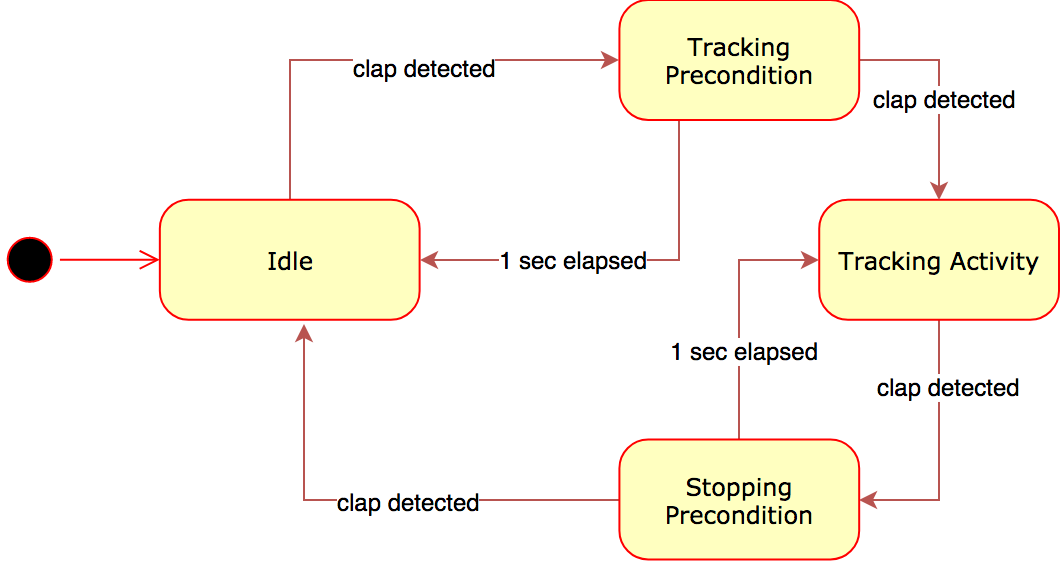
\includegraphics[width=1.0\linewidth]{./imgs/statemachine.png}
	\caption{UML State Chart Diagram for the state machine}
	\label{statemachine}
\end{figure}

There are a total of four states in which the app can be in. 
\begin{itemize}
\item Idle: The initial state when starting the app and the state after an activity tracking has been completed.
\item StartPrecondition: If the app is in the idle state and a clap is detected, the state machine switches to this state. When switching to this state, a timer is started which defines the time window in which the second clap must occur in order to switch the state to TrackingActivity. If the timer expires before another clap is detected, the state machine switches back to the idle state.
\item TrackingActivity: After a second clap is detected while the timer of the start precondition has not yet elapsed, the state machine changes to this state and starts capturing the time by saving a time stamp.
\item StoppingPrecondition: If the state machine is in the TrackingActivity state and a clap occurs, then the state machine switches to this state, which behaves in the same way as the StartingPrecondition, except that on a successful second clap, it changes to the idle state and the tracking of the current activity is ended.
\end{itemize}

\subsection{Architecture}
\label{sec:org393d659}
This Chapter describes the architecture for the Digital Life Tracking App. The following figure \ref{class-diagram} shows the class diagram with the most important classes:

\begin{figure}[H]
	\centering
	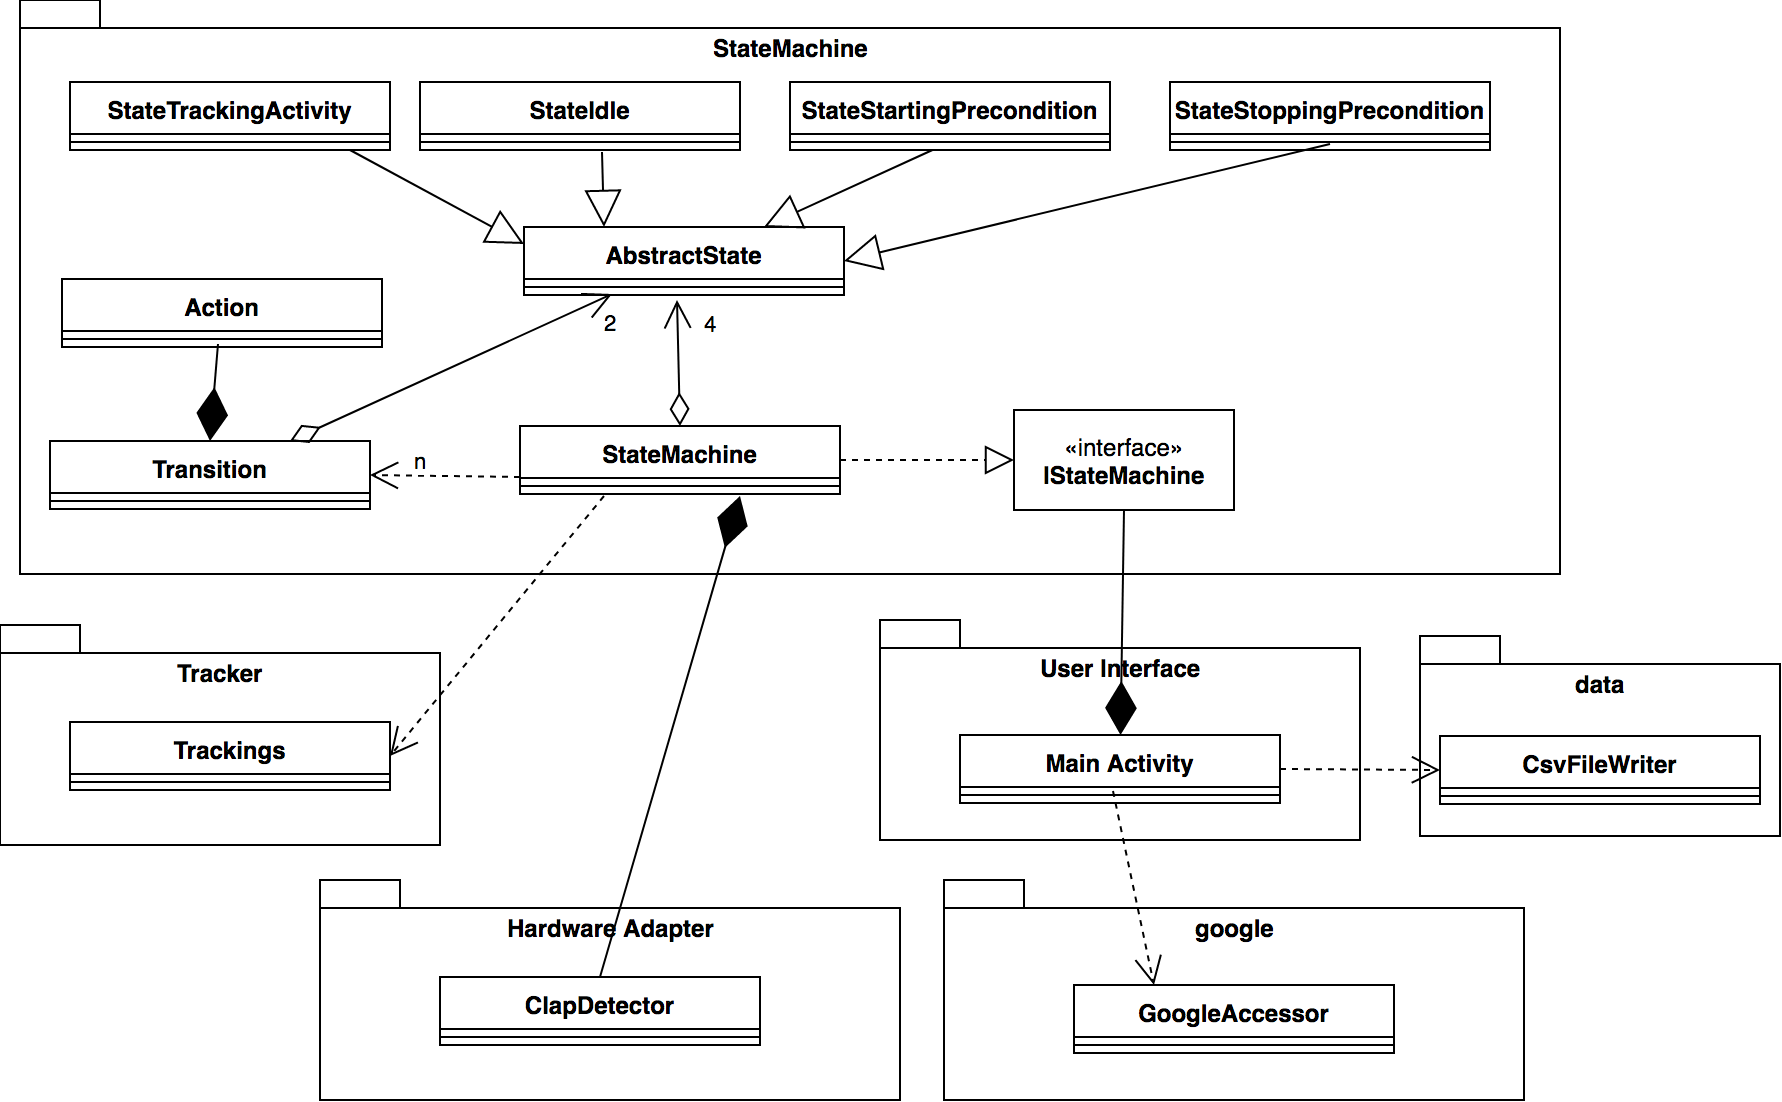
\includegraphics[width=1.0\linewidth]{./imgs/classUML.png}
	\caption{UML Class Diagram}
	\label{class-diagram}
\end{figure}

\subsubsection{StateMachine}
\label{sec:org9ea54c6}

The state machine presented in the previous chapter takes care of the logic 
of the app and switches back and forth between states when registering the corresponding event. 
The Statemachine class is the center of the package of the same name and performs the tasks described in the previous chapter.
It holds instances of all four states and a configuration of all possible transitions between the individual states.
Each transition in the configuration is also linked to an action that determines the event that triggers 
the transition. Each transition also defines the previous state and the next state.
When a transition is triggered, other operations are also executed that either adapt UI elements to the new 
state or execute other functions that are important for parts of the business logic.

\subsubsection{Hardware Adapter}
\label{sec:org0a1c43f}
The hardware adapter package includes the ClapDetector class, which uses the SmartPhone's microphone to listen 
for ambient sounds and tries to detect a clap from the recorded frequencies. When a clap is detected, 
a handler is triggered in the state machine. This triggers a transition between two states in the state machine.
This is illustrated in figure \ref{statemachine}.

\subsubsection{Tracker}
\label{sec:orgd2cdde2}

One of the operations triggered by the transitions in the state machine is to start or stop the tracker, 
which stores the activities of the user together with the measured times in a list.

\subsubsection{User Interface}
\label{sec:org2938786}

The User Interface package contains the main activity of the app, which initializes the other functions of 
the program including the state machine. The goal was that the Main Activity class should contain as little 
business logic as possible. The business logic has been implemented almost completely in the state machine. 
If possible, the class should only provide and control the UI elements of the app. It also controls the permissions 
request to the user, which the user must give in order for the apps to work properly.

\subsubsection{Google}
\label{sec:org3d3dca0}
This package contains the GoogleAccessor class, which was initially designed to upload the test data stored on the 
smartphone via the CSVWriter class to the Google Cloud. Once enough data has been collected, this functionality has 
been disabled for the release of the app. The reason for this was that access to the cloud required signed APK, 
which had nothing to do with the pure functionality of the app. Commenting out the code of this feature should 
avoid unnecessary problems when starting the app.

\subsubsection{Data}
\label{sec:orgdeb052b}
The data package contains the CsvFileWriter class, which stores the frequencies recorded by the ClapDetector in 
CSV files on the memory of the smartphone. This functionality was used during development to collect test data 
for later analysis.

\subsection{UI Design}
\label{sec:orgc19d2ea}
In order to make faster progress in the development of the app, a user interface was initially implemented, which was designed for the developers' tasks. The interface should display the transitions between the individual states of the state machine and the events in an output field as logs. The interface should also support the collection of test data that was later uploaded to the Google Cloud for analysis. 
\\\\
At the same time, a design for the future user interface was also created, which was intended to replace the development interface after completion of the basic functionalities of the app. The following figure \ref{mockups} shows mockups for both user interfaces:
\begin{figure}[H]
	\centering
	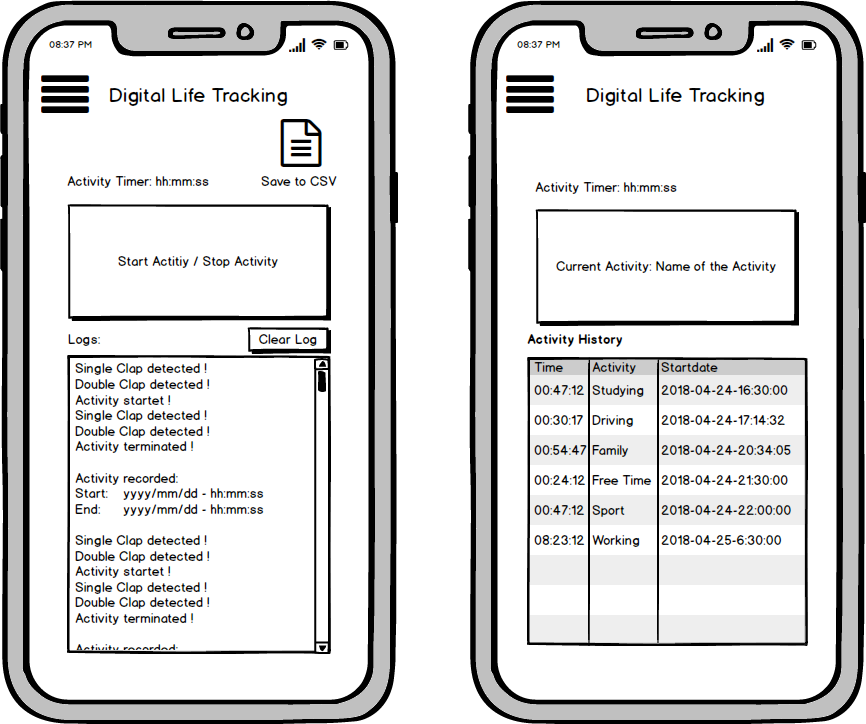
\includegraphics[width=1.0\linewidth]{./imgs/mock.png}
	\caption{Mockups for development UI (left) and for the final UI (right)}
	\label{mockups}
\end{figure}
The finished user interface should display a timer for the currently tracked activity and the name of the activity. In addition, it should display the last completed activities in a cronologically arranged list, whereby the name of the activity, the start time, as well as the duration of the activation should be visible.
\\
Since there was not enough time to implement the actual user interface during development later on, the app only has the development UI as it is currently available. Figure \ref{ui-screenshot} shows a screenshot of the actual development UI:
\begin{figure}[H]
	\centering
	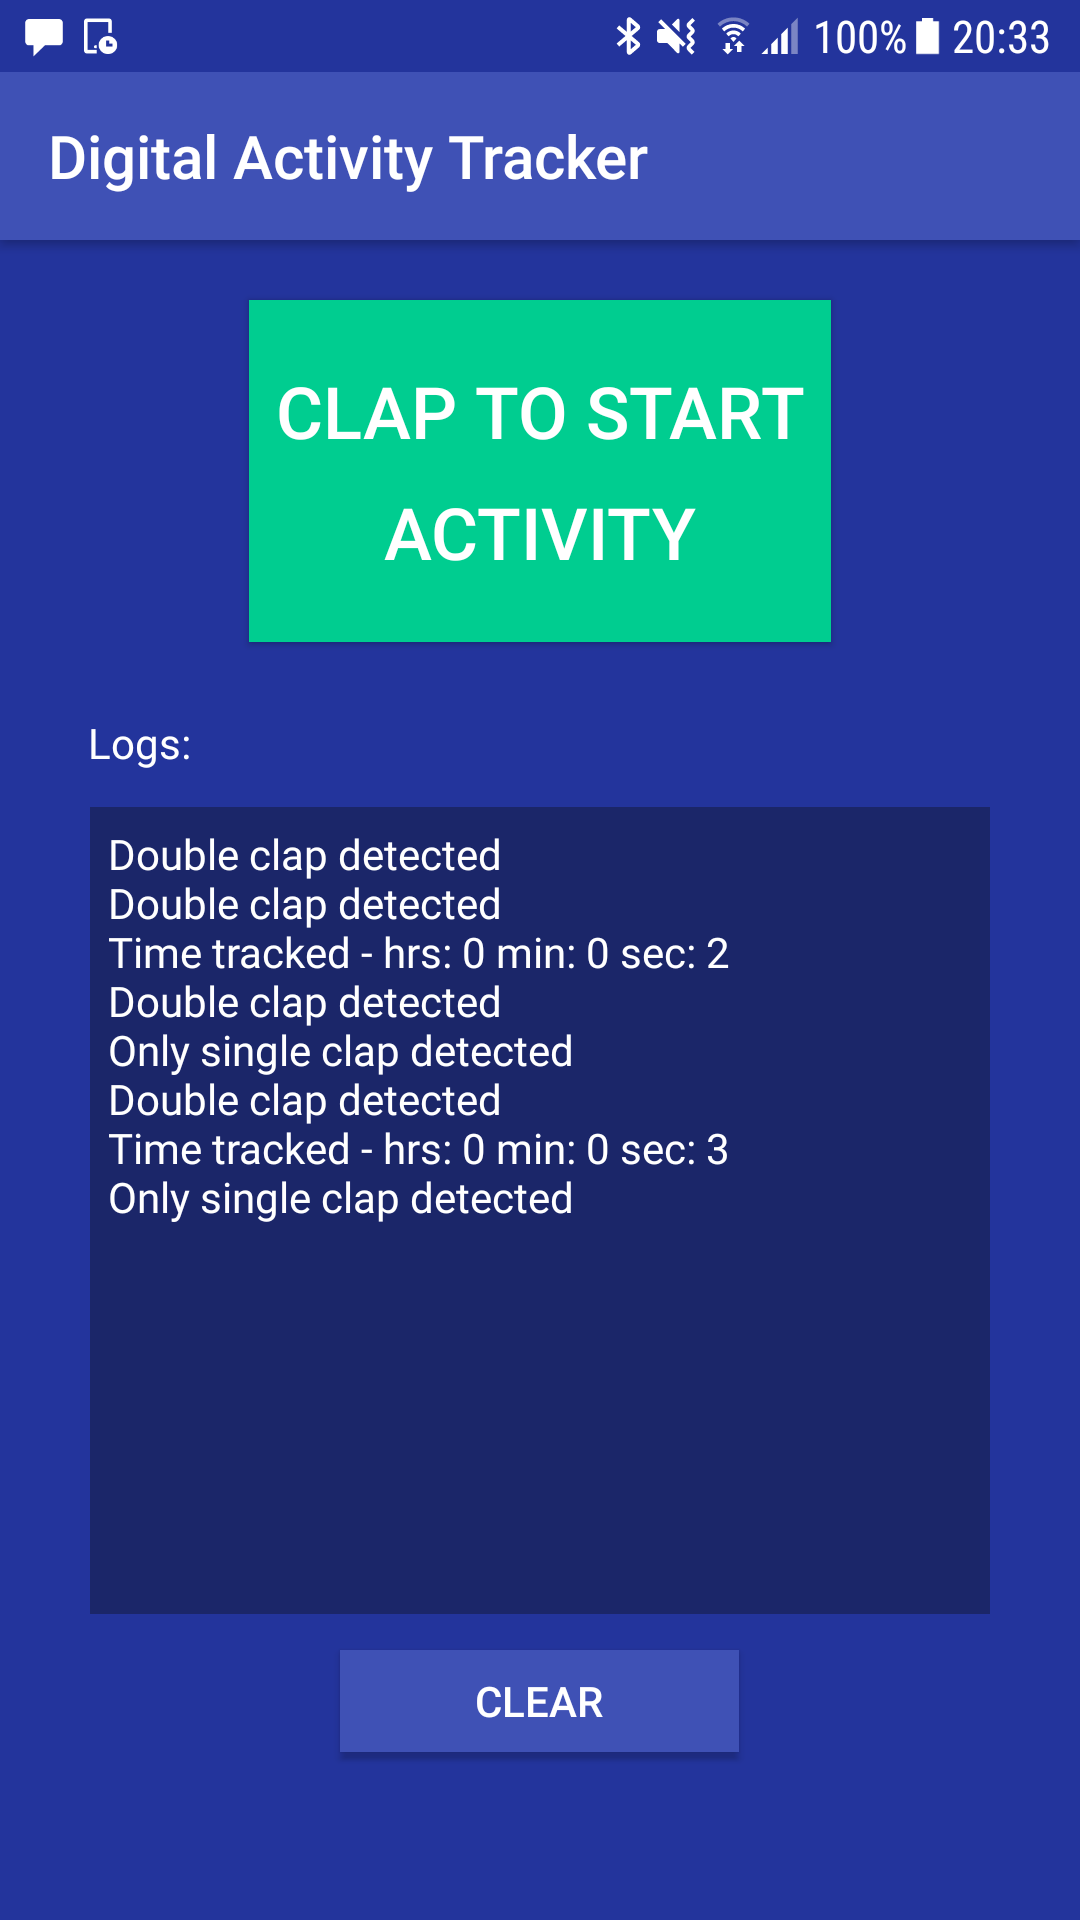
\includegraphics[width=0.5\linewidth]{./imgs/uiScreenshot.png}
	\caption{Screenshot of the development UI}
	\label{ui-screenshot}
\end{figure}